\section{Résultats} \label{sec: resultats}

\subsection{Trajectoires} \label{subsec: res_trajectories}
    Soit les figures \ref{fig: traj_lorenz}, \ref{fig: traj_rossler} et
    \ref{fig: traj_bouali} qui présentent les résultats pour la simulation des
    attracteurs (Lorenz, Rössler et Bouali) définis mathématiquement dans la
    section \fullref{sec: theory}. On voit sur lesdites figures la trajectoires
    d'une particule de masse unité dans les systèmes dynamiques dissipatifs
    représentés par les différents attracteurs. Étonnement, les trajectoires
    montrées sur ces figures ne semble pas du tout chaotiques, et se
    rapprochent d'arrangements très bien organisés voir même prédictibles. Une
    fois de plus, la subtilité réside dans la sensibilité de ces systèmes aux
    conditions initiales. Il est d'ailleurs à noter que ces figures sont des
    trajectoires qui proviennent d'\textbf{une seule} position initiale à
    chaque fois. Pour voir à quel point ces attracteurs sont chaotiques ou non,
    nous devrions exécuter la simulation pour une multitude de coordonnées
    initiales et ainsi observer la divergence très précoce entre les solutions.
    Un bon indicateur de signature chaotique est le spectre de Lyapunov et
    c'est pourquoi nous allons analyser ce spectre en utilisant les mêmes
    trajectoires attractives. \\

    Il est également intéressant d'observer sur les figures
    \ref{fig: traj_lorenz}, \ref{fig: traj_rossler} et \ref{fig: traj_bouali}
    que le théorème d'unicité des solutions d'équations différentielles
    ordinaires est vérifié \cite{uniqueness}. On observe effectivement aucun
    croisement dans les trajectoires obtenues.

\subsection{Spectre de Lyapunov} \label{subsec: res_lyapunov}
    Considérons les figures \ref{fig : lyaps_lorenz},
    \ref{fig : lyaps_rossler} et \ref{fig : lyaps_bouali}, sur lesquelles ont
    observe le calcul du spectre de Lyapunov en fonction du temps pour les
    trajectoires attractives discutées dans la section
    \fullref{subsec: res_trajectories}. Il est intéressant d'observer la
    précieuse utilisation de l'algorithme de convergence epsilon introduit dans
    la section \fullref{subsec: convergence}. La convergence est pertinente et
    permet bien d'identifier le comportement à long terme
    ($\lim_{t\to\infty}\lambda_i(t)$) du spectre de Lyapunov pour la
    trajectoire des attracteurs étudiés. \\

    On remarque premièrement, pour tous les attracteurs, que l'exposant de
    Lyapunov maximal $\lambda_1$ est positif. Comme introduit dans la section
    \fullref{subsec: lyapunov}, il s'agit-là d'une signature typique de chaos.
    Mathématiquement, cela signifie que dans la direction associée à l'exposant
    $\lambda_1$ deux trajectoires voisines divergent exponentiellement
    rapidement dans le temps et donc que de toutes petites perturbations
    peuvent mener à des trajectoires très différentes. On peut ici faire un
    lien avec la contraction/expansion de l'espace des phases modélisée par
    l'évolution du volume de la sphère unitaire $U$ vis-à-vis du signe obtenu
    pour les composantes du spectre de Lyapunov. \\

    Ensuite, on remarque que dans les résultats obtenus, deux des trois
    exposants sont négatifs. Cela signifie logiquement que deux trajectoires
    voisines tendent à converger au sein de l'attracteur et demeurer près l'une
    de l'autre. Physiquement, on peut aussi dire que des exposants négatifs
    indiquent que les systèmes étudiés sont dissipatifs (perdent de l'énergie
    au cours du temps) et donc qu'il est normal d'observer la convergence de
    certaines trajectoires comme par exemple lorsque l'on étudie un oscillateur
    harmonique amorti. \\

    Finalement, on voit que certains des exposants de Lyapunov sont nuls. Ces
    derniers n'impliquent pas de comportement chaotique particuliers. On peut
    conclure que mathématiquement, une perturbation d'une trajectoire ayant un
    exposant de Lyapunov nul peut se voir diverger mais seulement de façon
    logarithmique. On appelle ce phénomène:
    \textit{comportement quasi-périodique}.

\onecolumngrid
\vspace{2cm}

    \begin{figure}[h!]
        \centering
        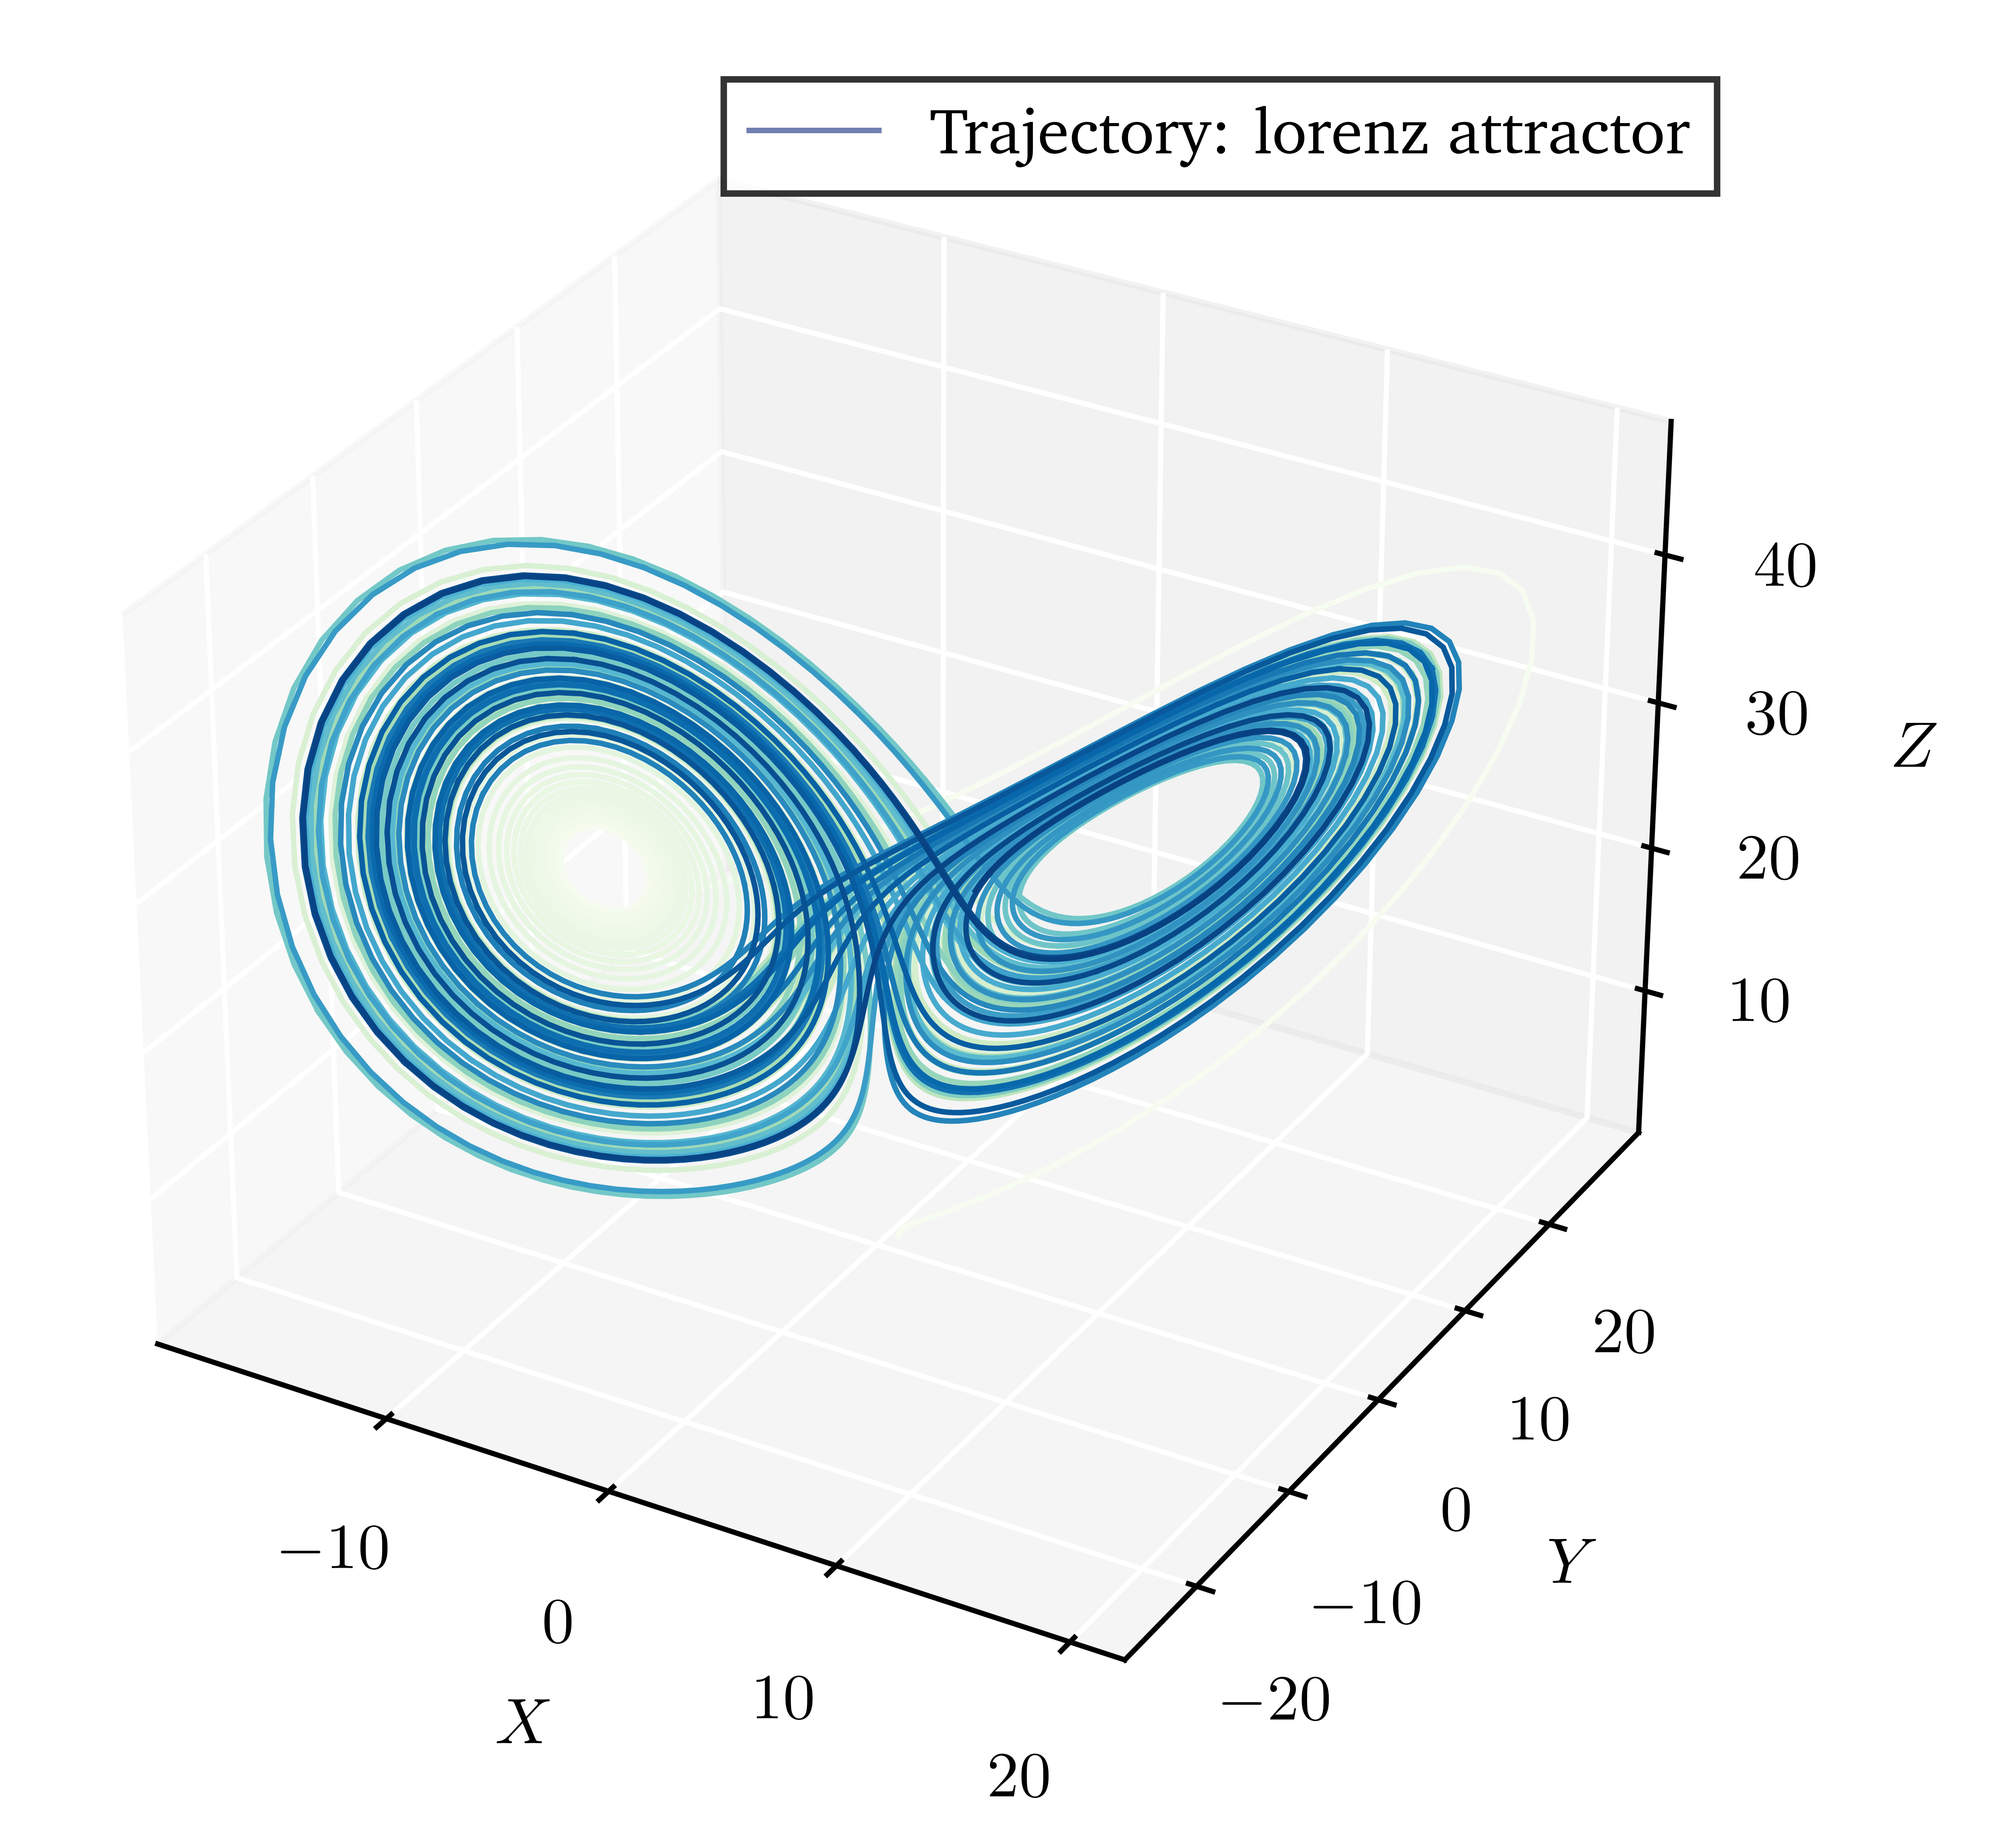
\includegraphics[scale=0.6]{figs/trajectories/traj_lorenz.png}
        \caption{Trajectoire obtenue pour la simulation d'une particule de
        masse unité dans le bassin d'attraction de l'attracteur de Lorenz ayant
    comme position initiale $\bm{r}_0 = (1, 0, -1)$ ainsi que pour un temps de
100 secondes avec un pas de $h = 0.01$.}
        \label{fig: traj_lorenz}
    \end{figure}
    \vspace{1cm}
    \begin{figure}[h!]
        \centering
        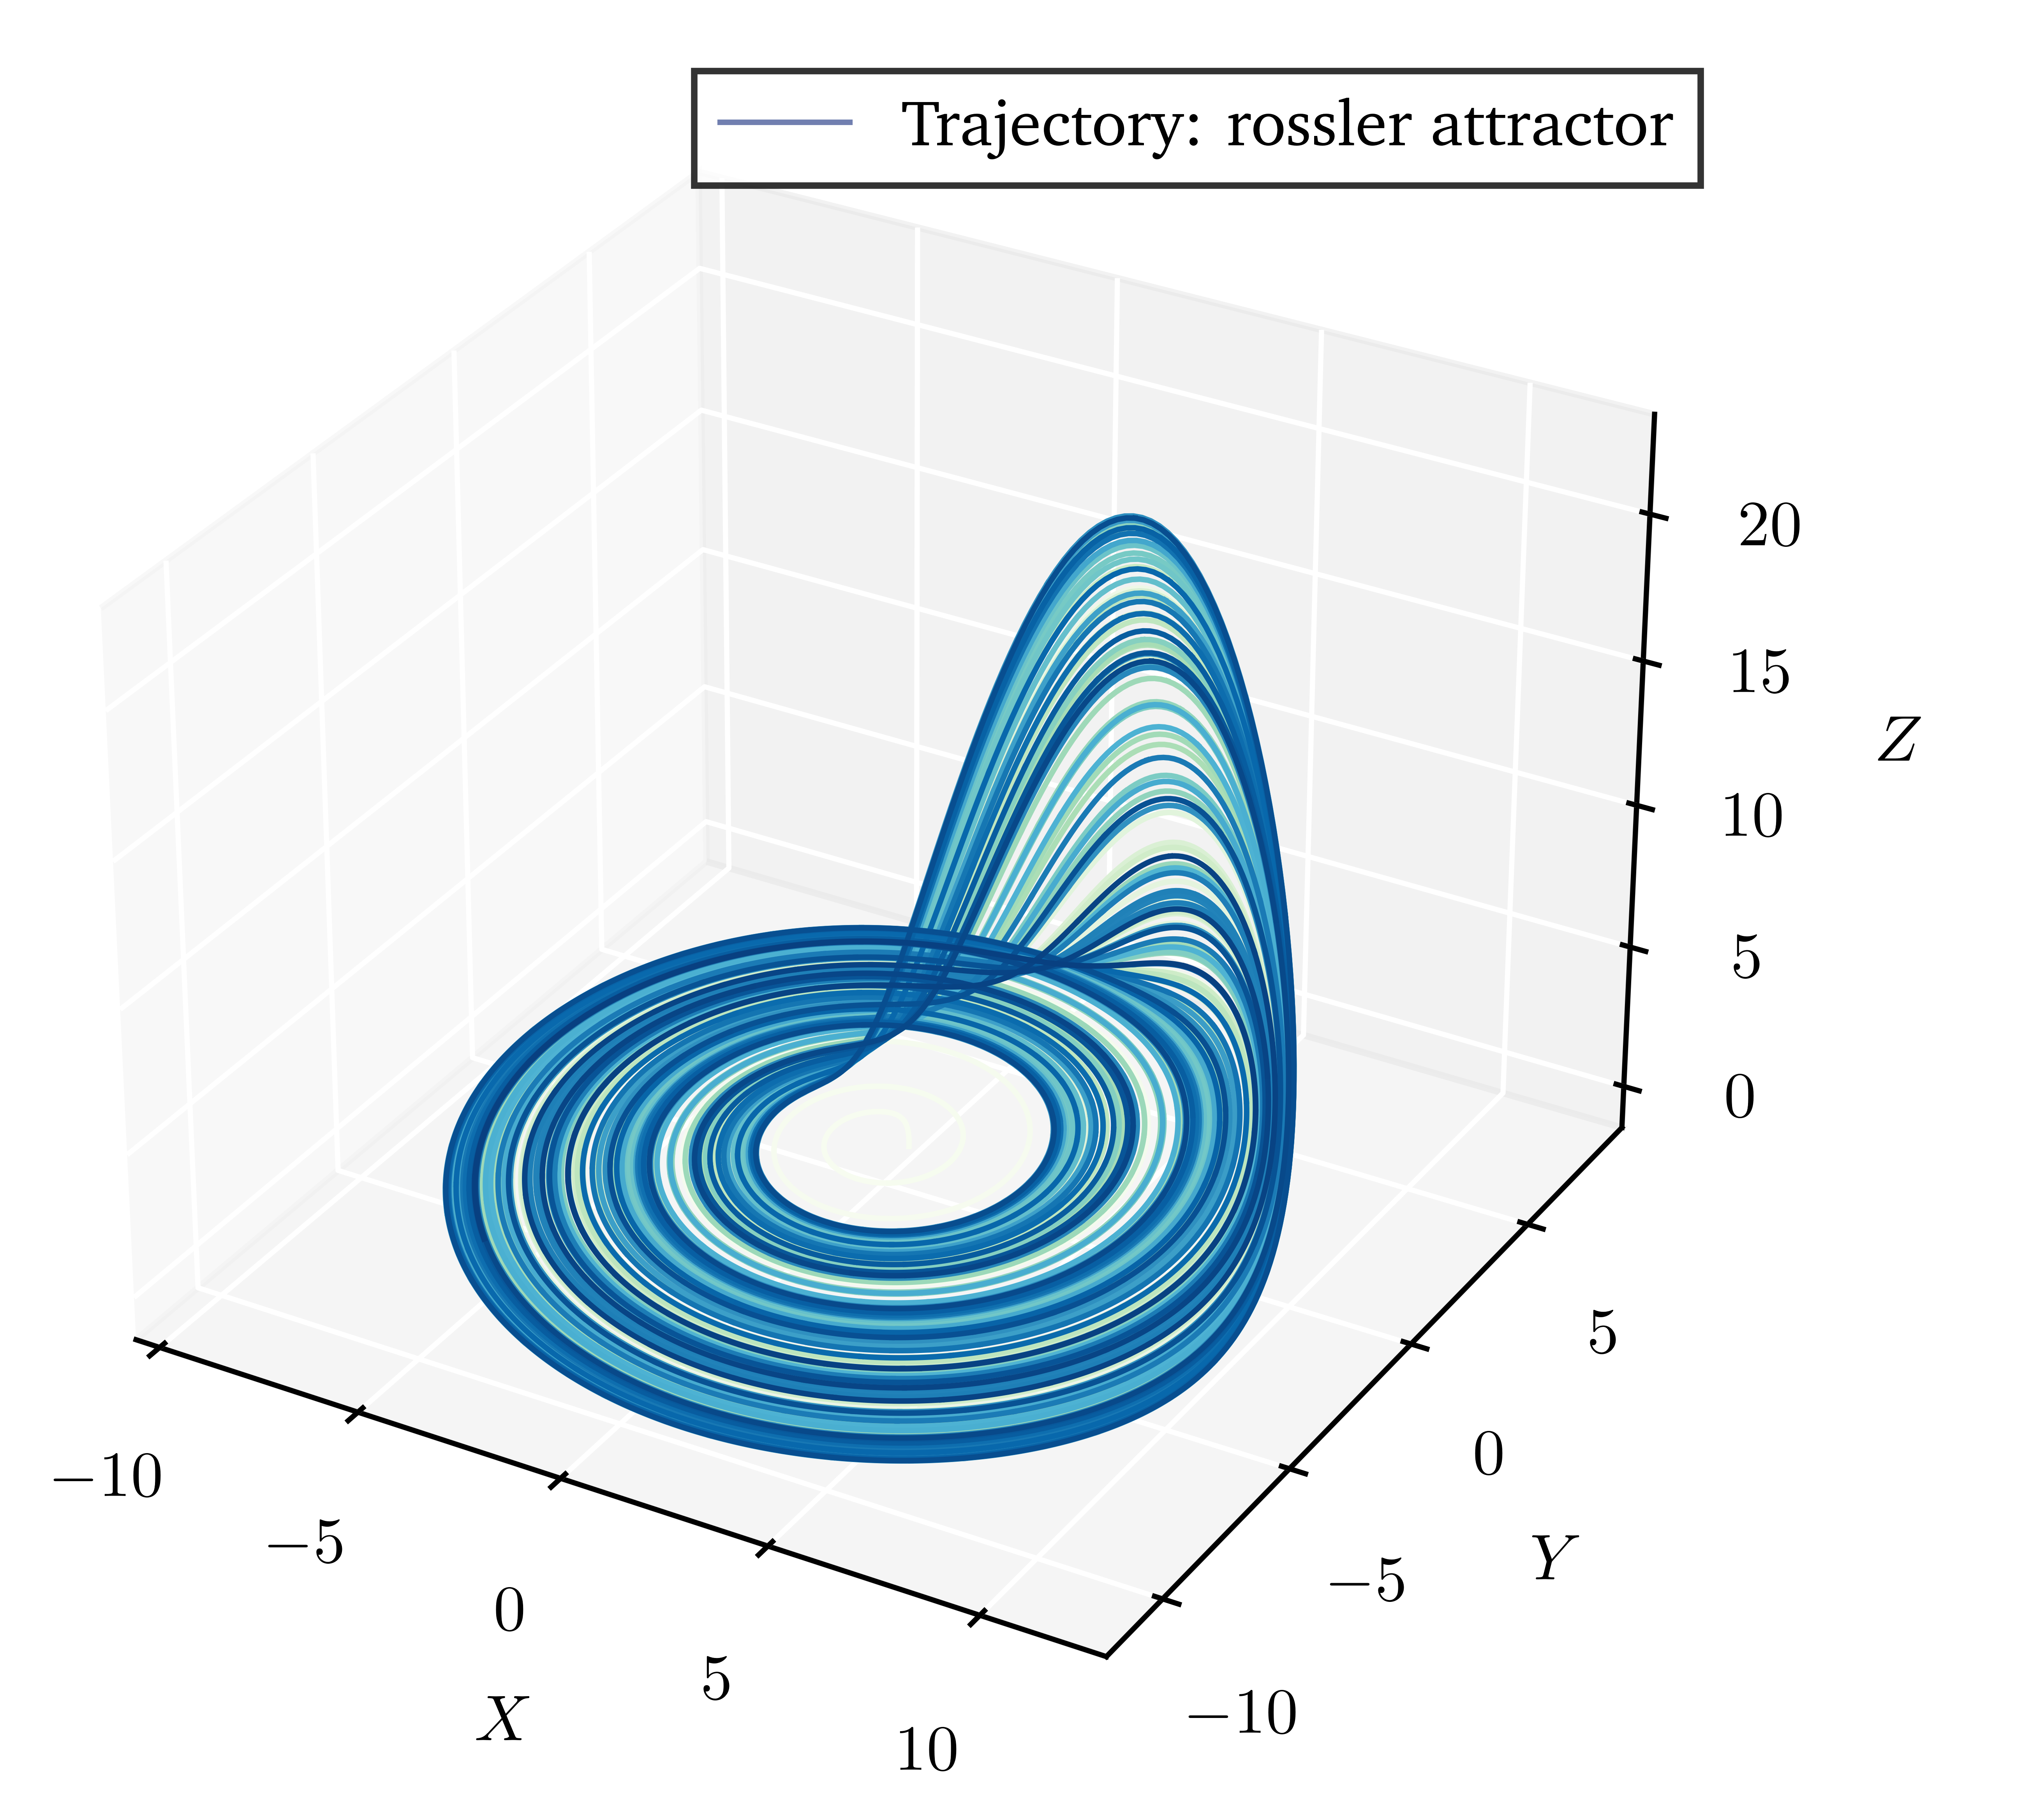
\includegraphics[scale=0.6]{figs/trajectories/traj_rossler.png}
        \caption{Trajectoire obtenue pour la simulation d'une particule de
        masse unité dans le bassin d'attraction de l'attracteur de Rössler ayant
    comme position initiale $\bm{r}_0 = (1, 1, -1)$ ainsi que pour un temps de
1000 secondes avec un pas de $h = 0.001$.}
        \label{fig: traj_rossler}
    \end{figure}

\clearpage

    \begin{figure}[h!]
        \centering
        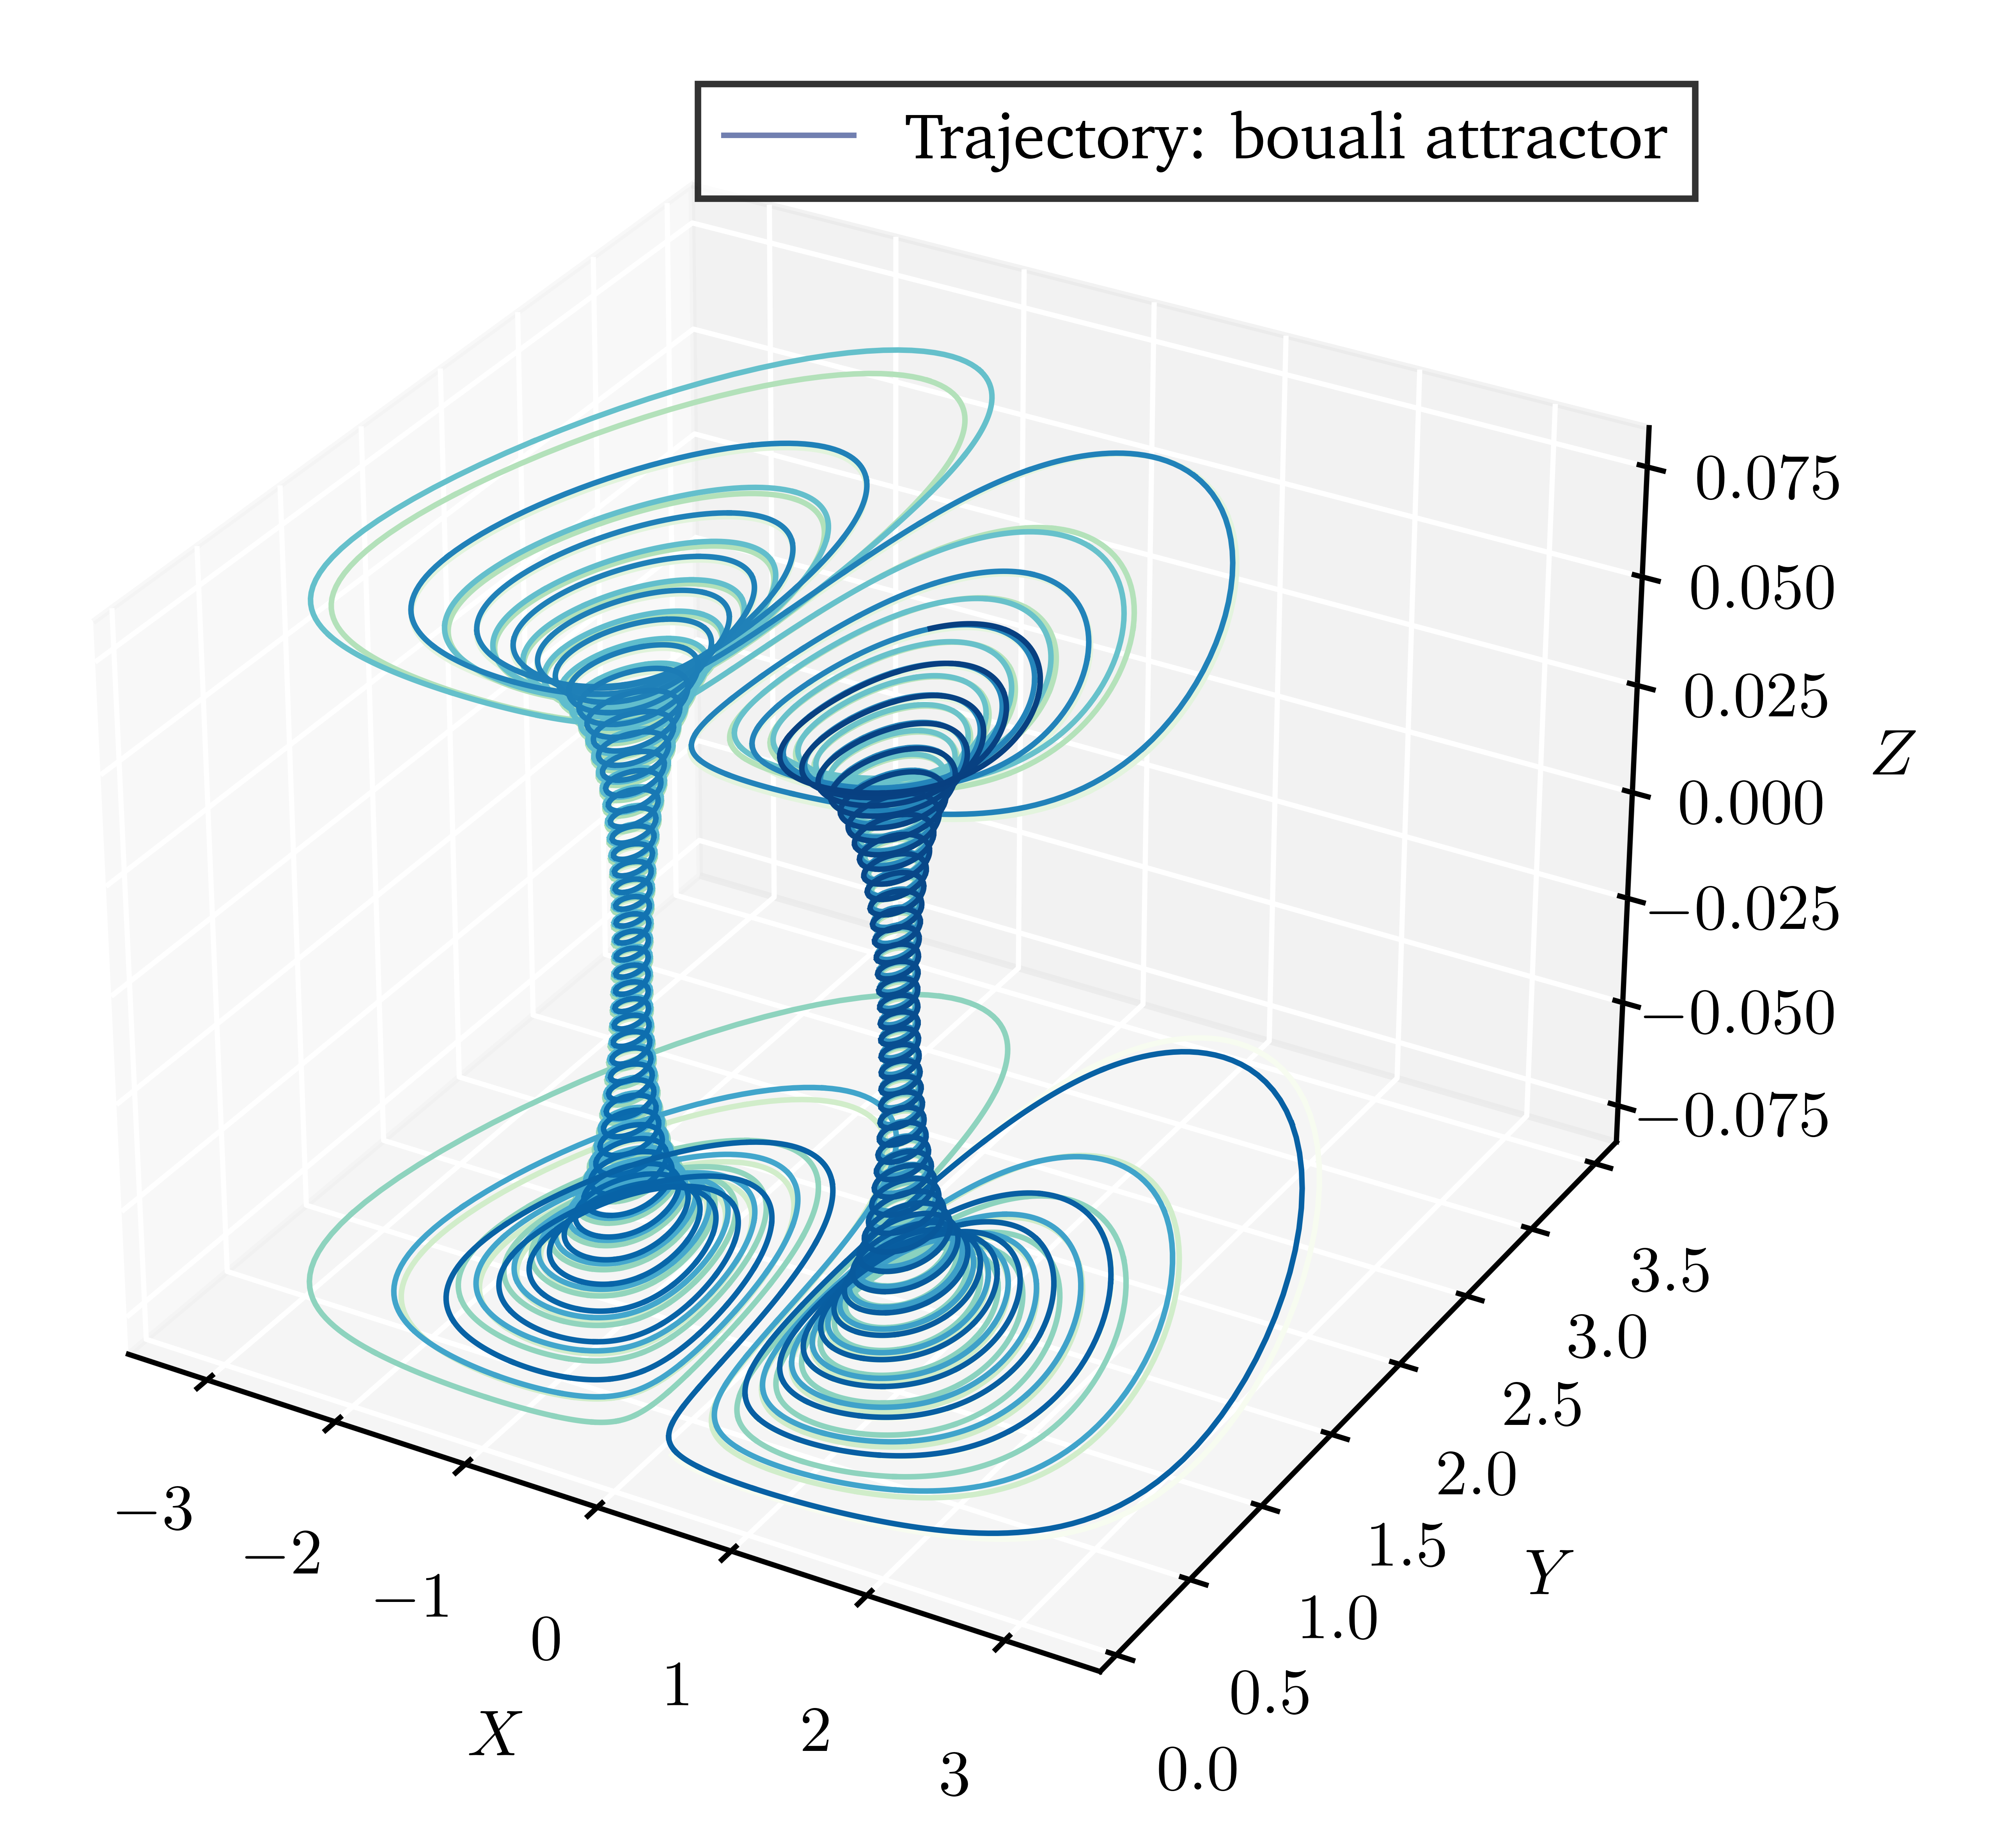
\includegraphics[scale=0.5]{figs/trajectories/traj_bouali.png}
        \caption{Trajectoire obtenue pour la simulation d'une particule de
        masse unité dans le bassin d'attraction de l'attracteur de Bouali ayant
    comme position initiale $\bm{r}_0 = (0.2, 0.2, -0.08)$ ainsi que pour un
temps de 1000 secondes avec un pas de $h = 0.001$.}
        \label{fig: traj_bouali}
    \end{figure}

    \begin{figure}[h!]
        \centering
        \begin{minipage}{0.49\textwidth}
          \centering
          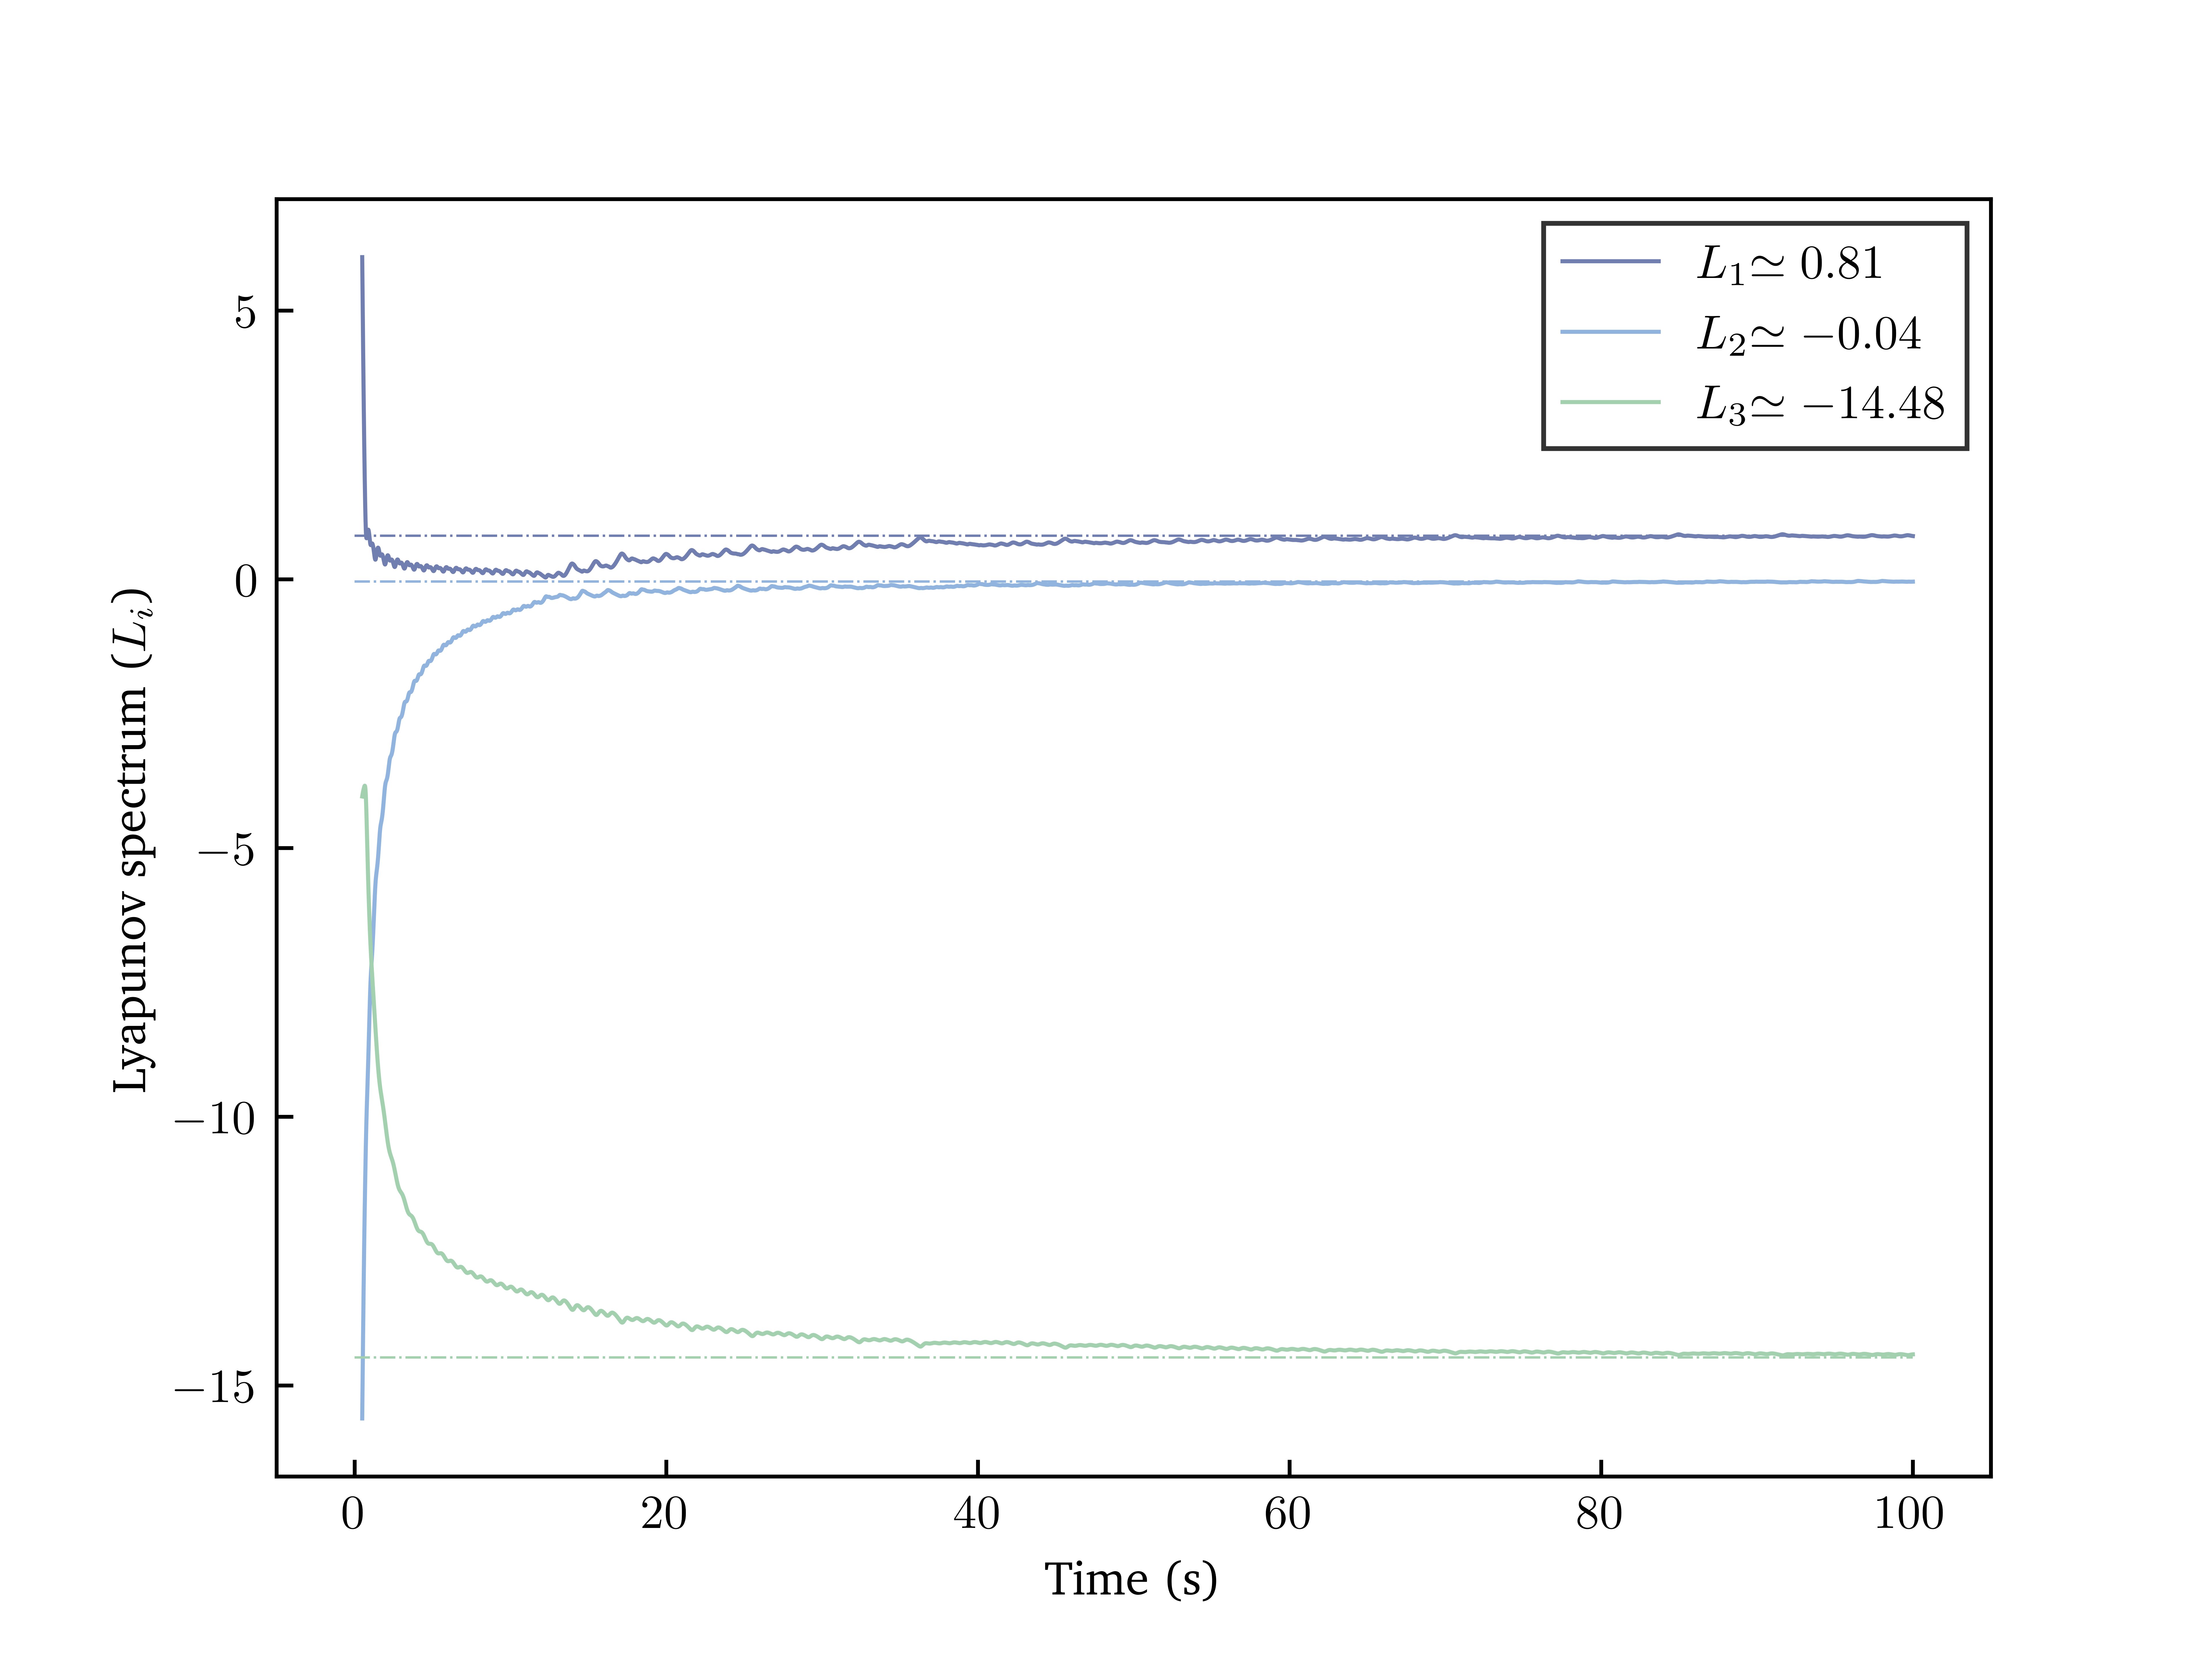
\includegraphics[scale = 0.4]{figs/lyapunovs/lyap_lorenz.png}
          \subcaption{}
          \label{fig: lyap_lorenz}
        \end{minipage}
        \begin{minipage}{0.49\textwidth}
          \centering
          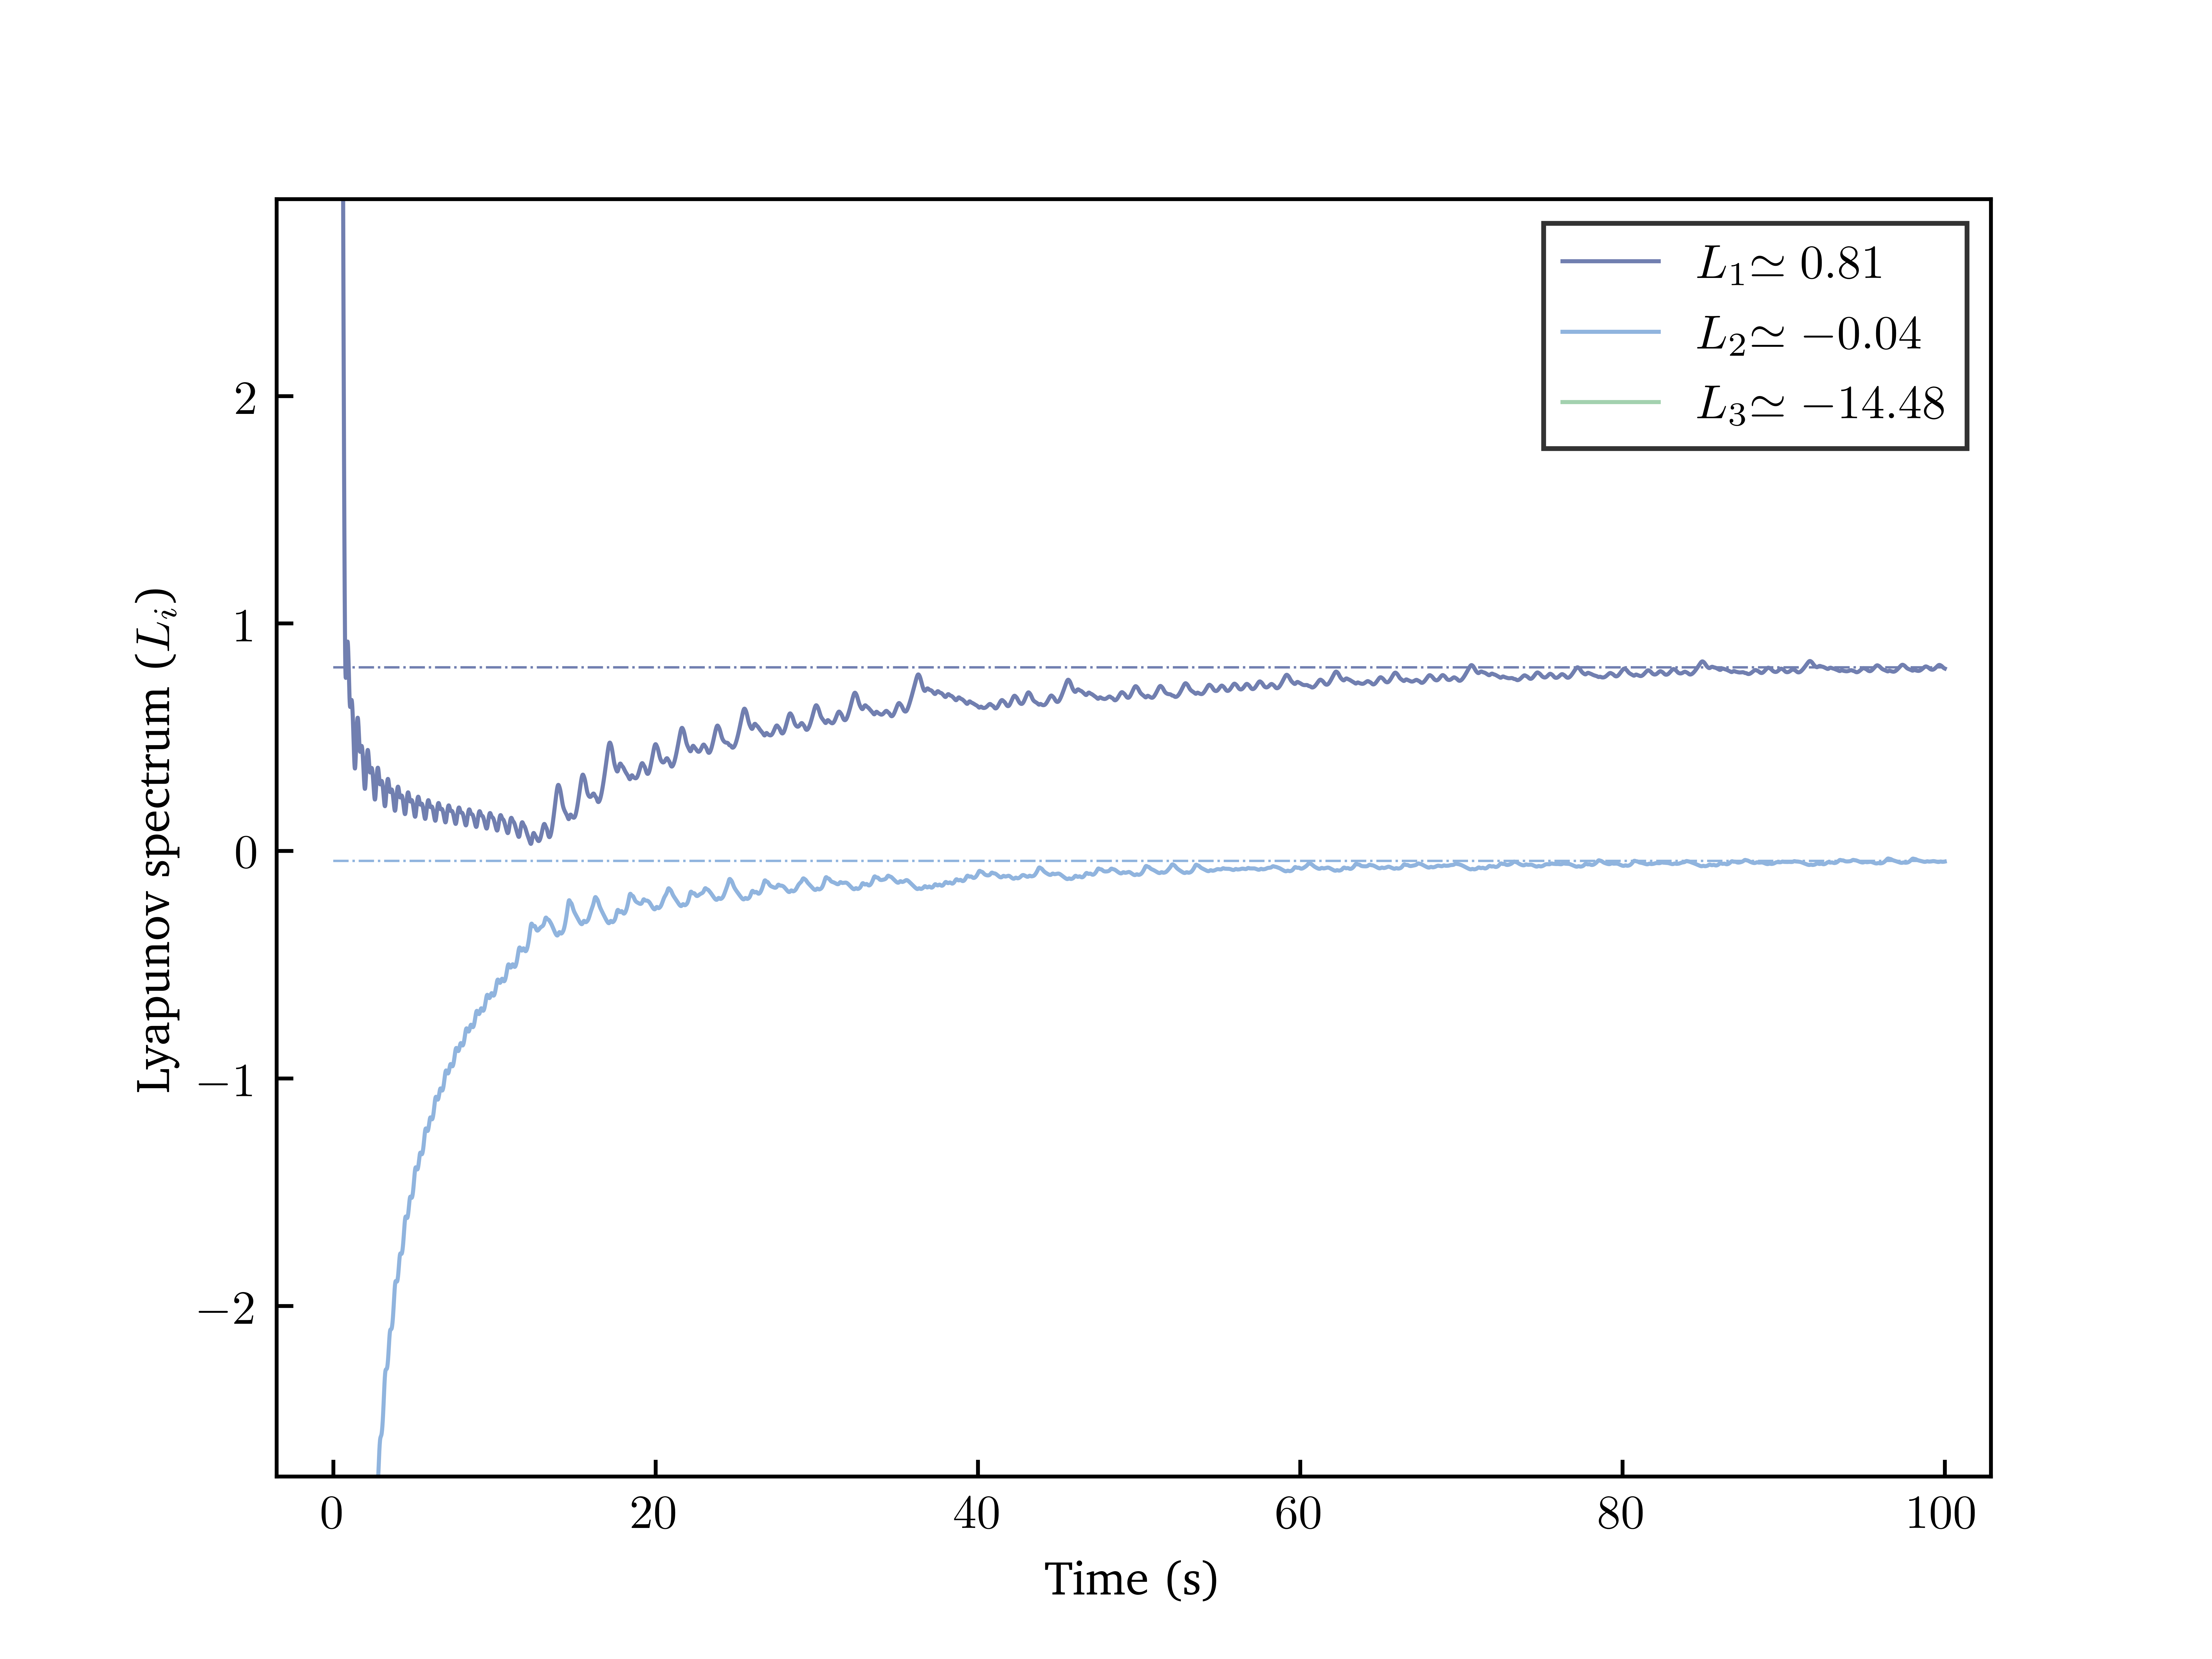
\includegraphics[scale = 0.4]{figs/lyapunovs/lyap_lorenz_zoom.png}
          \subcaption{}
          \label{fig: lyap_lorenz_zoom}
        \end{minipage}
        \caption{Spectre de Lyapunov ($\lambda_i\forall i\in\{1, 2, 3\}$) dans
        la simulation de l'attracteur de Lorenz. (a) Spectre complet. (b) Mise
    en évidence du comportement pour les exposants $\lambda_1$ et $\lambda_2$
étant donnée la superposition et le bruit.}
        \label{fig : lyaps_lorenz}
    \end{figure}

    \begin{figure}[h!]
        \centering
        \begin{minipage}{0.49\textwidth}
          \centering
          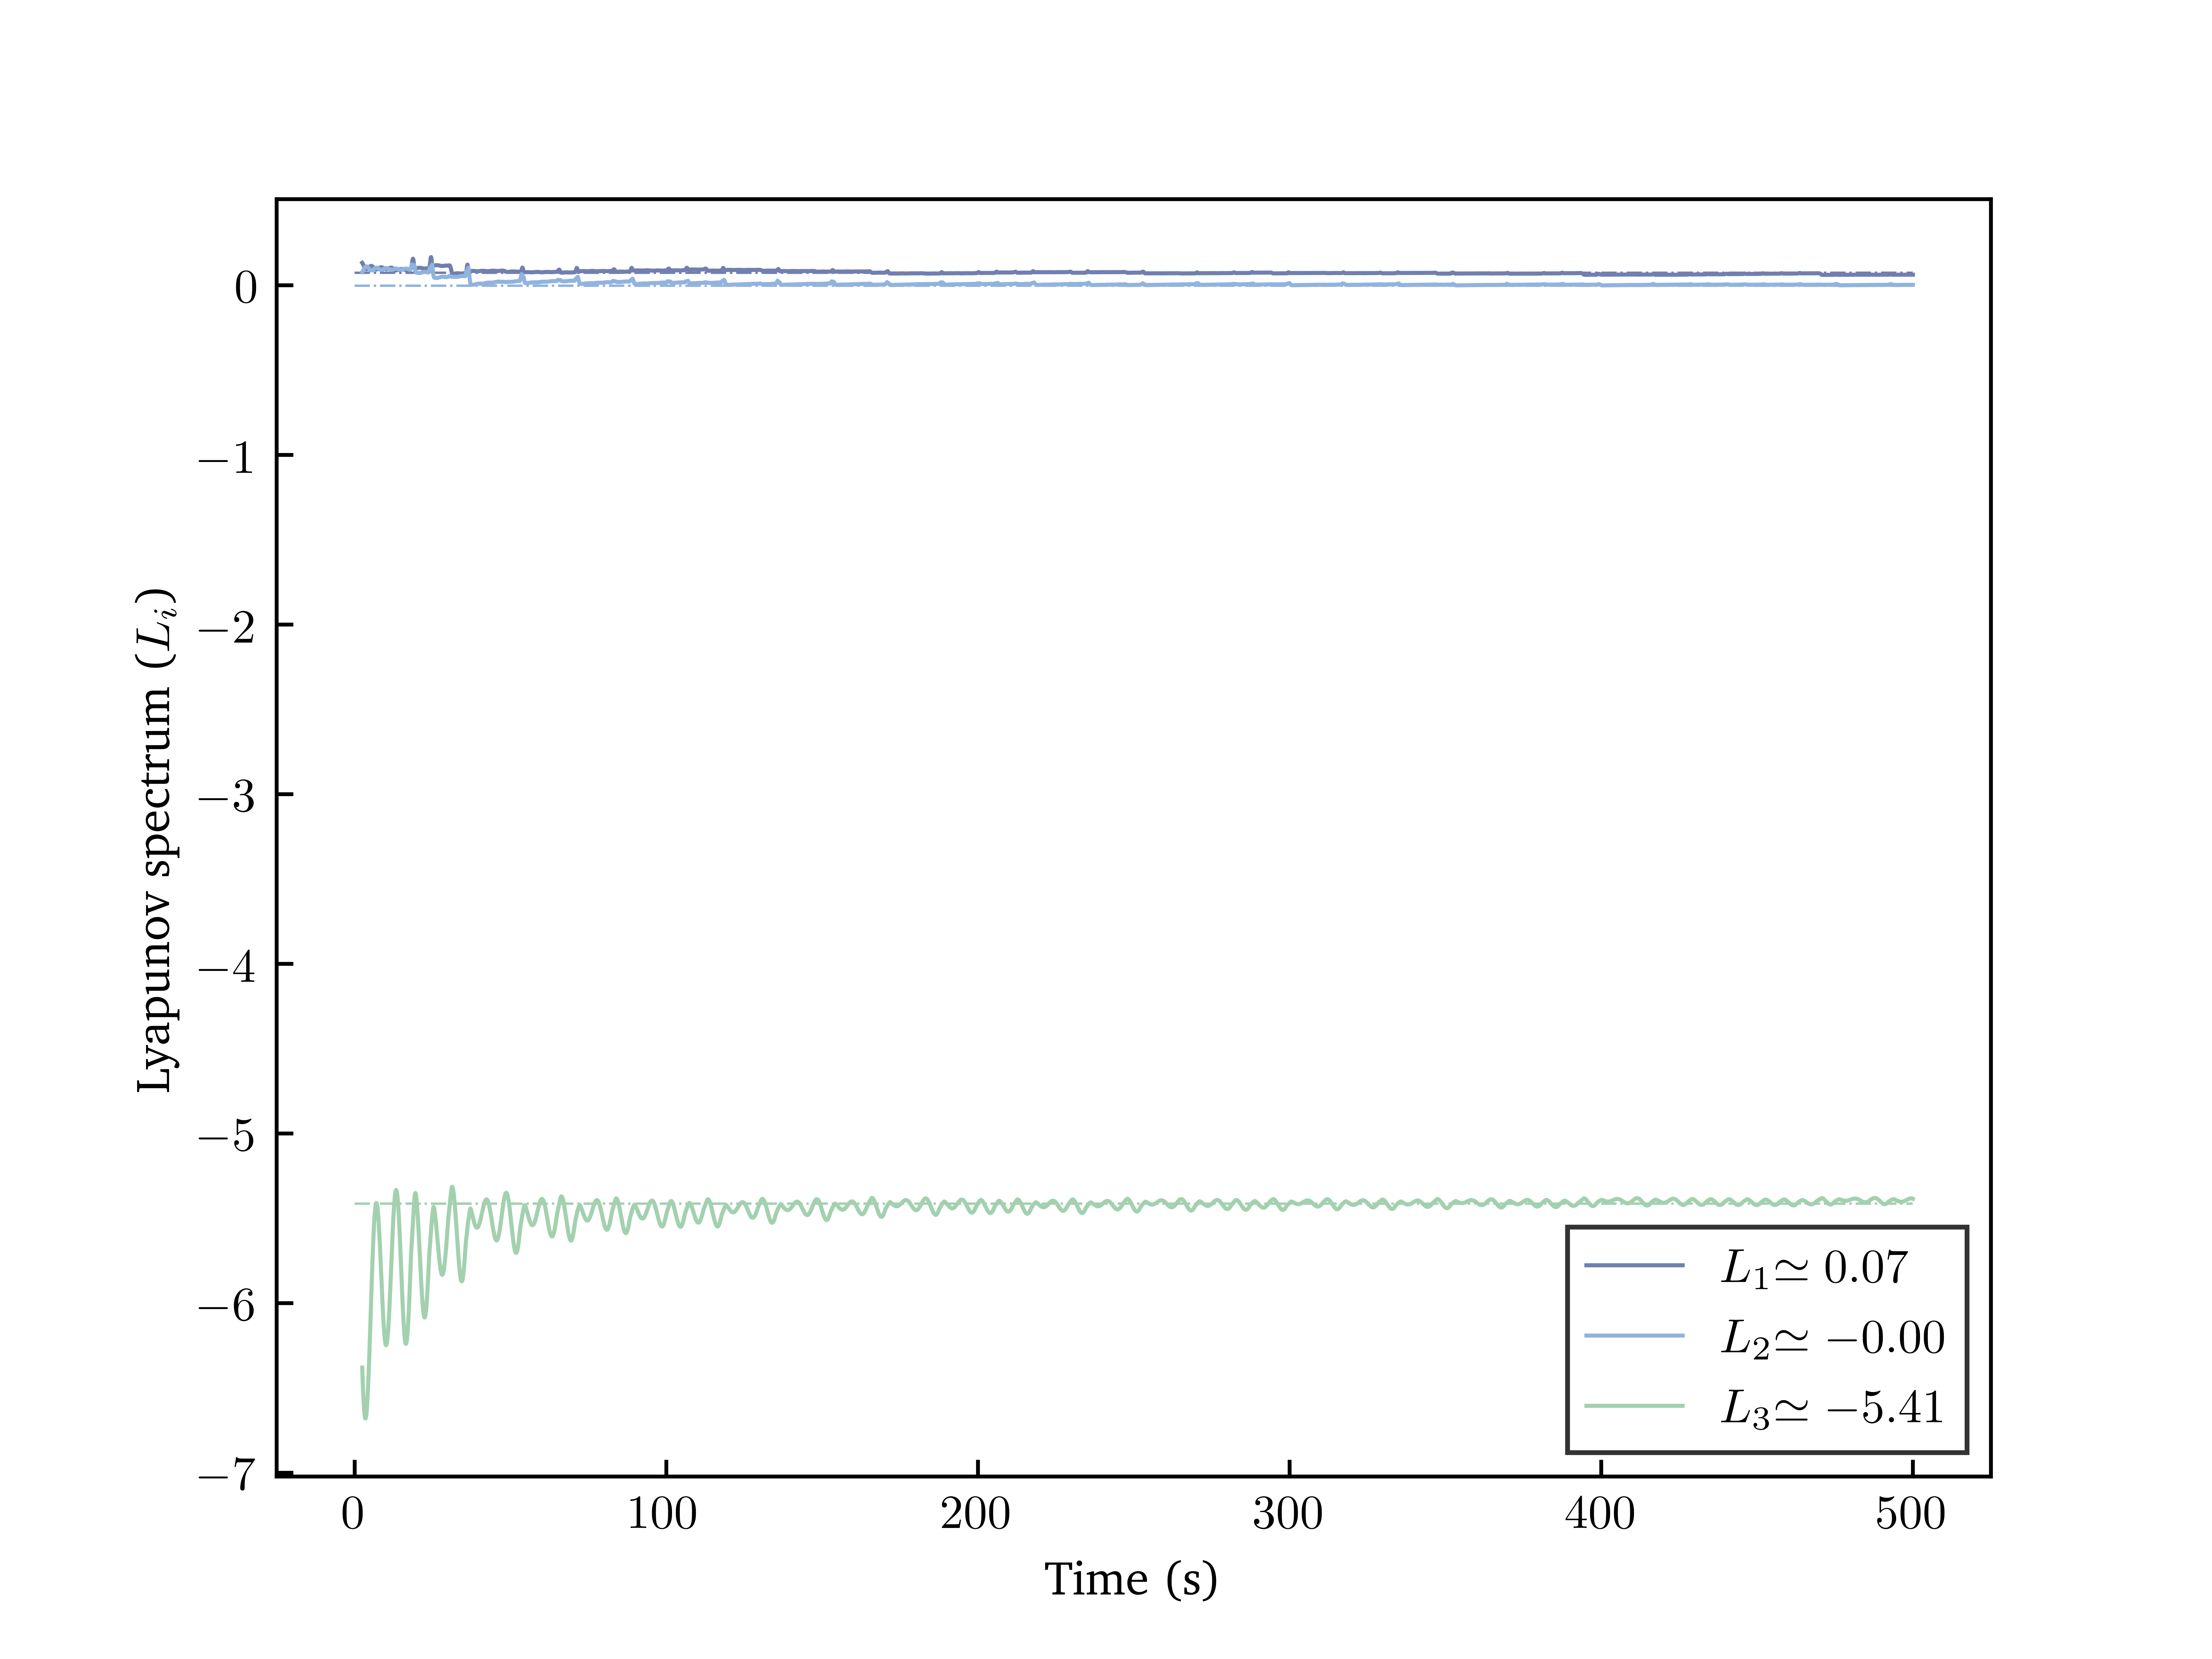
\includegraphics[scale = 0.4]{figs/lyapunovs/lyap_rossler.png}
          \subcaption{}
          \label{fig: lyap_rossler}
        \end{minipage}
        \begin{minipage}{0.49\textwidth}
          \centering
          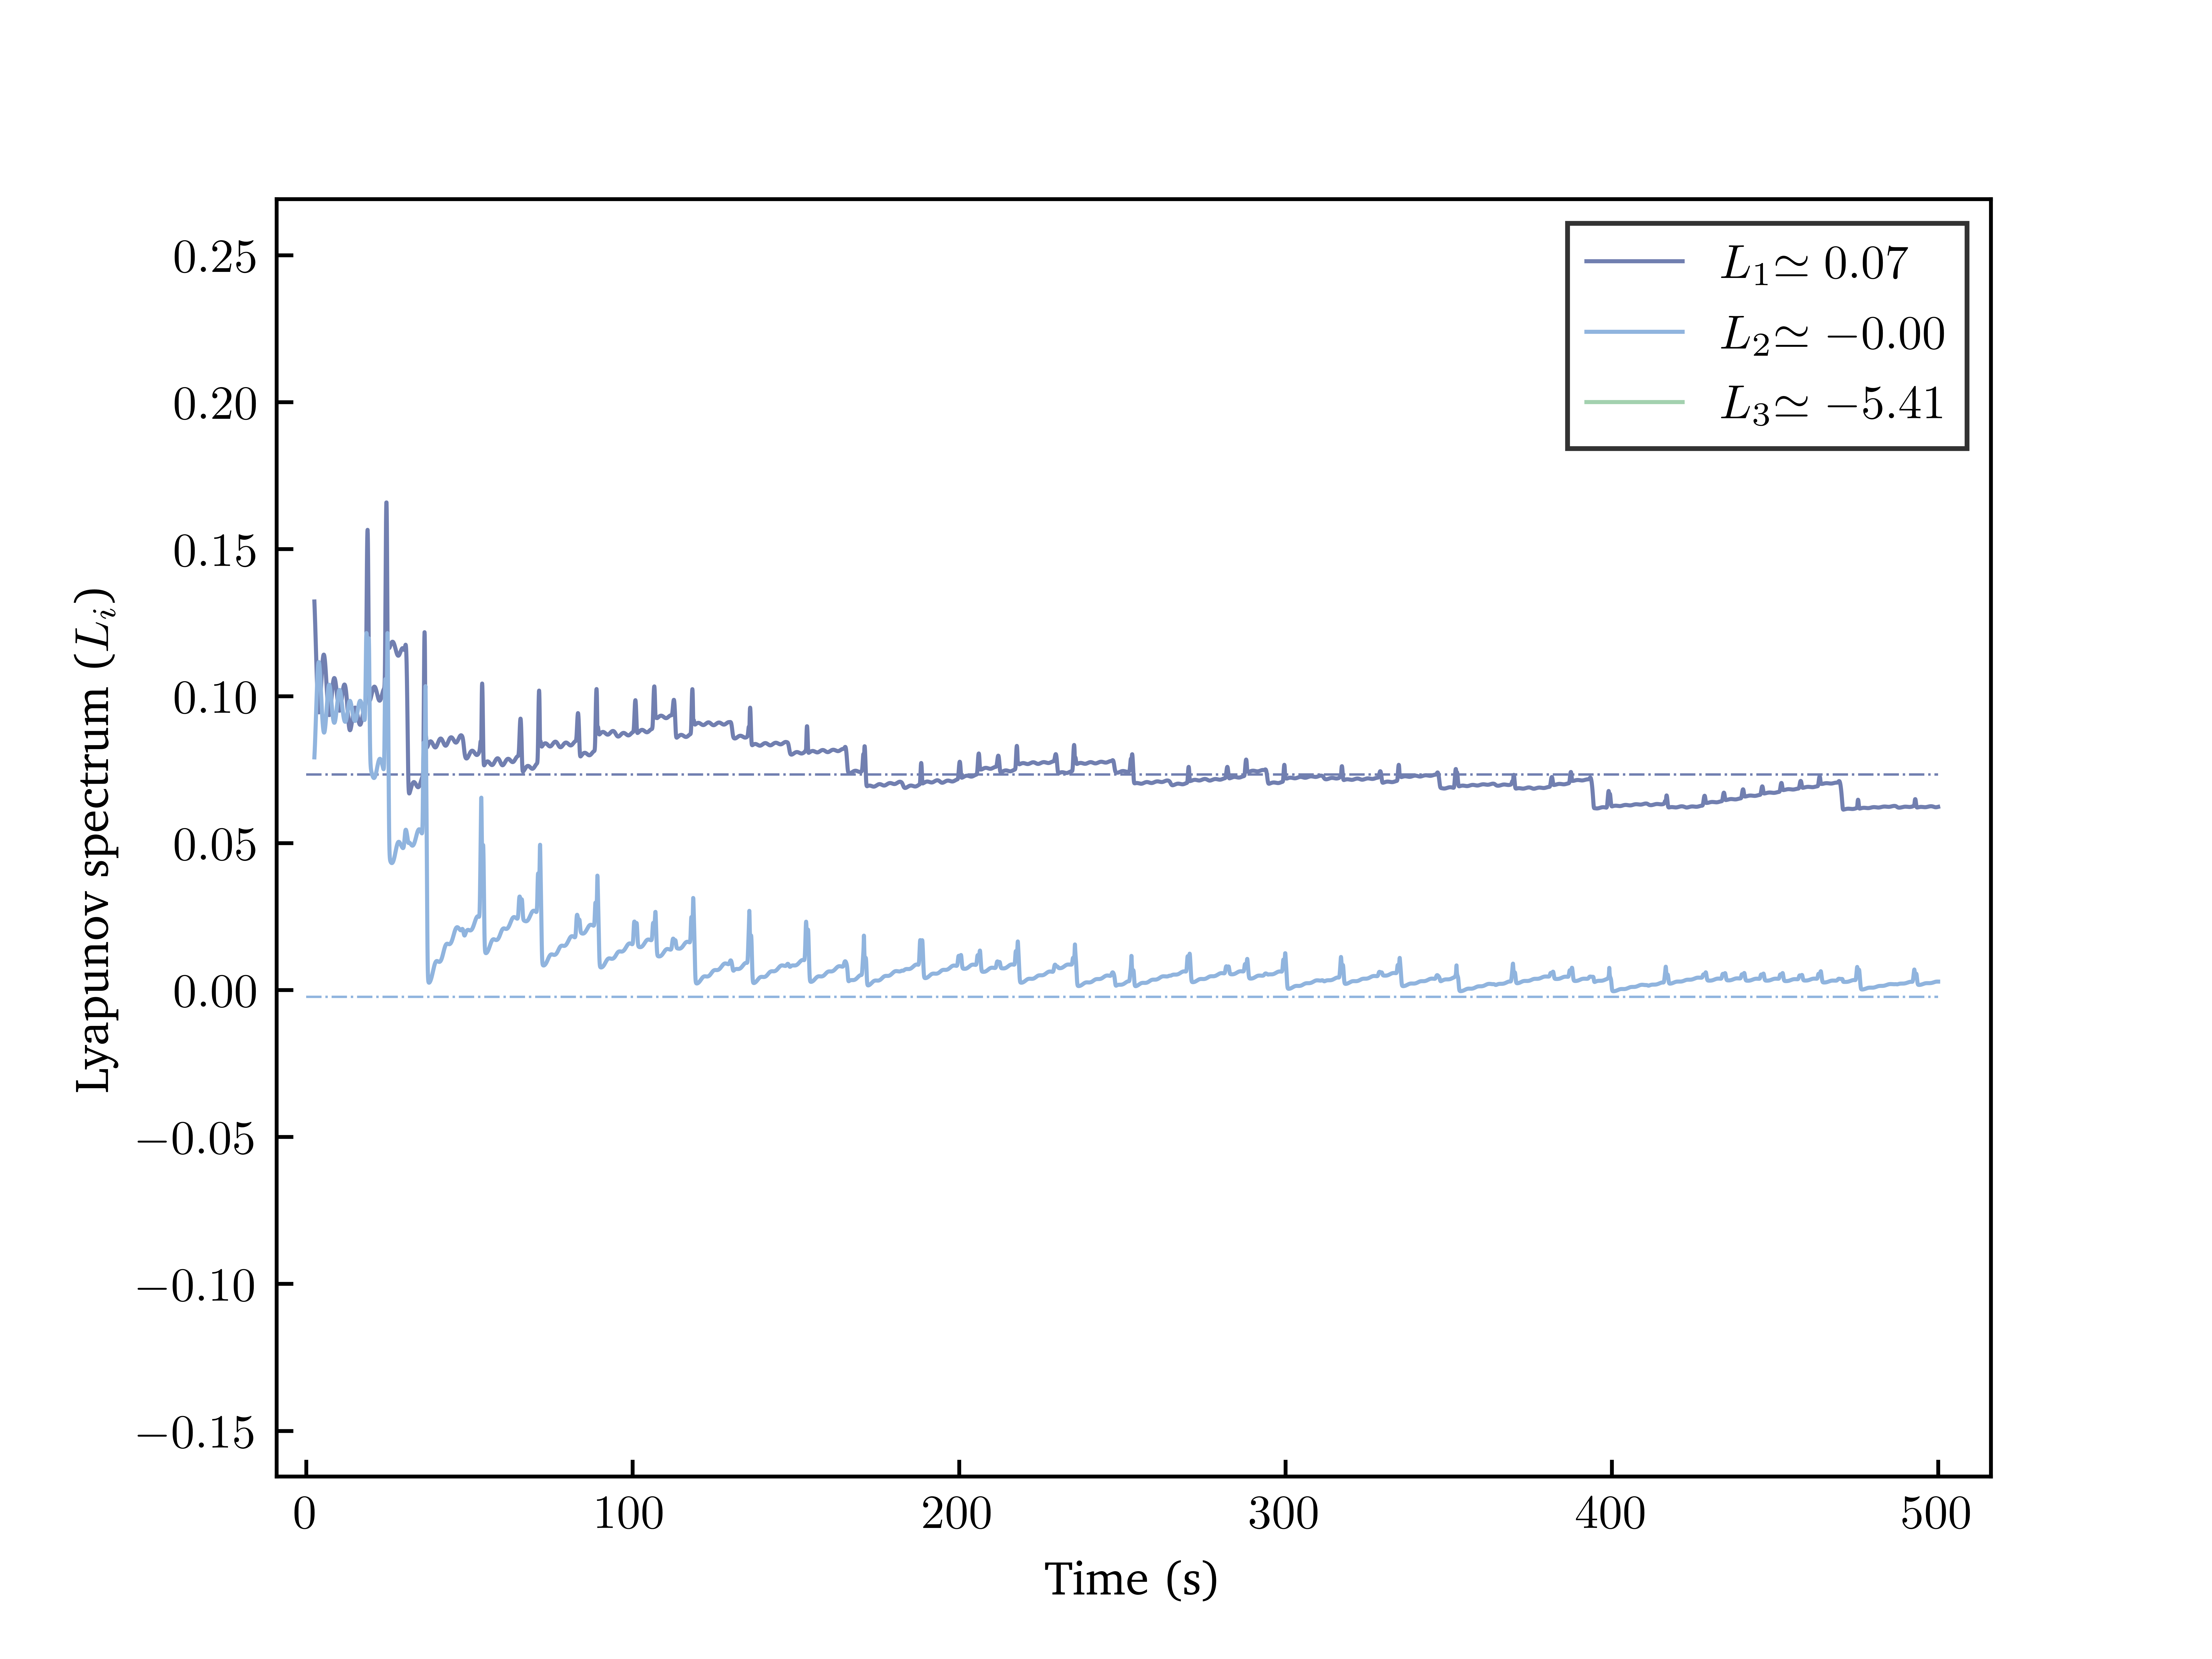
\includegraphics[scale = 0.4]{figs/lyapunovs/lyap_rossler_zoom.png}
          \subcaption{}
          \label{fig: lyap_rossler_zoom}
        \end{minipage}
        \caption{Spectre de Lyapunov ($\lambda_i\forall i\in\{1, 2, 3\}$) dans
        la simulation de l'attracteur de Rössler. (a) Spectre complet. (b) Mise
    en évidence du comportement pour les exposants $\lambda_1$ et $\lambda_2$
étant donnée la superposition et le bruit.}
        \label{fig : lyaps_rossler}
    \end{figure}

    \clearpage

    \begin{figure}[h!]
        \centering
        \begin{minipage}{0.49\textwidth}
          \centering
          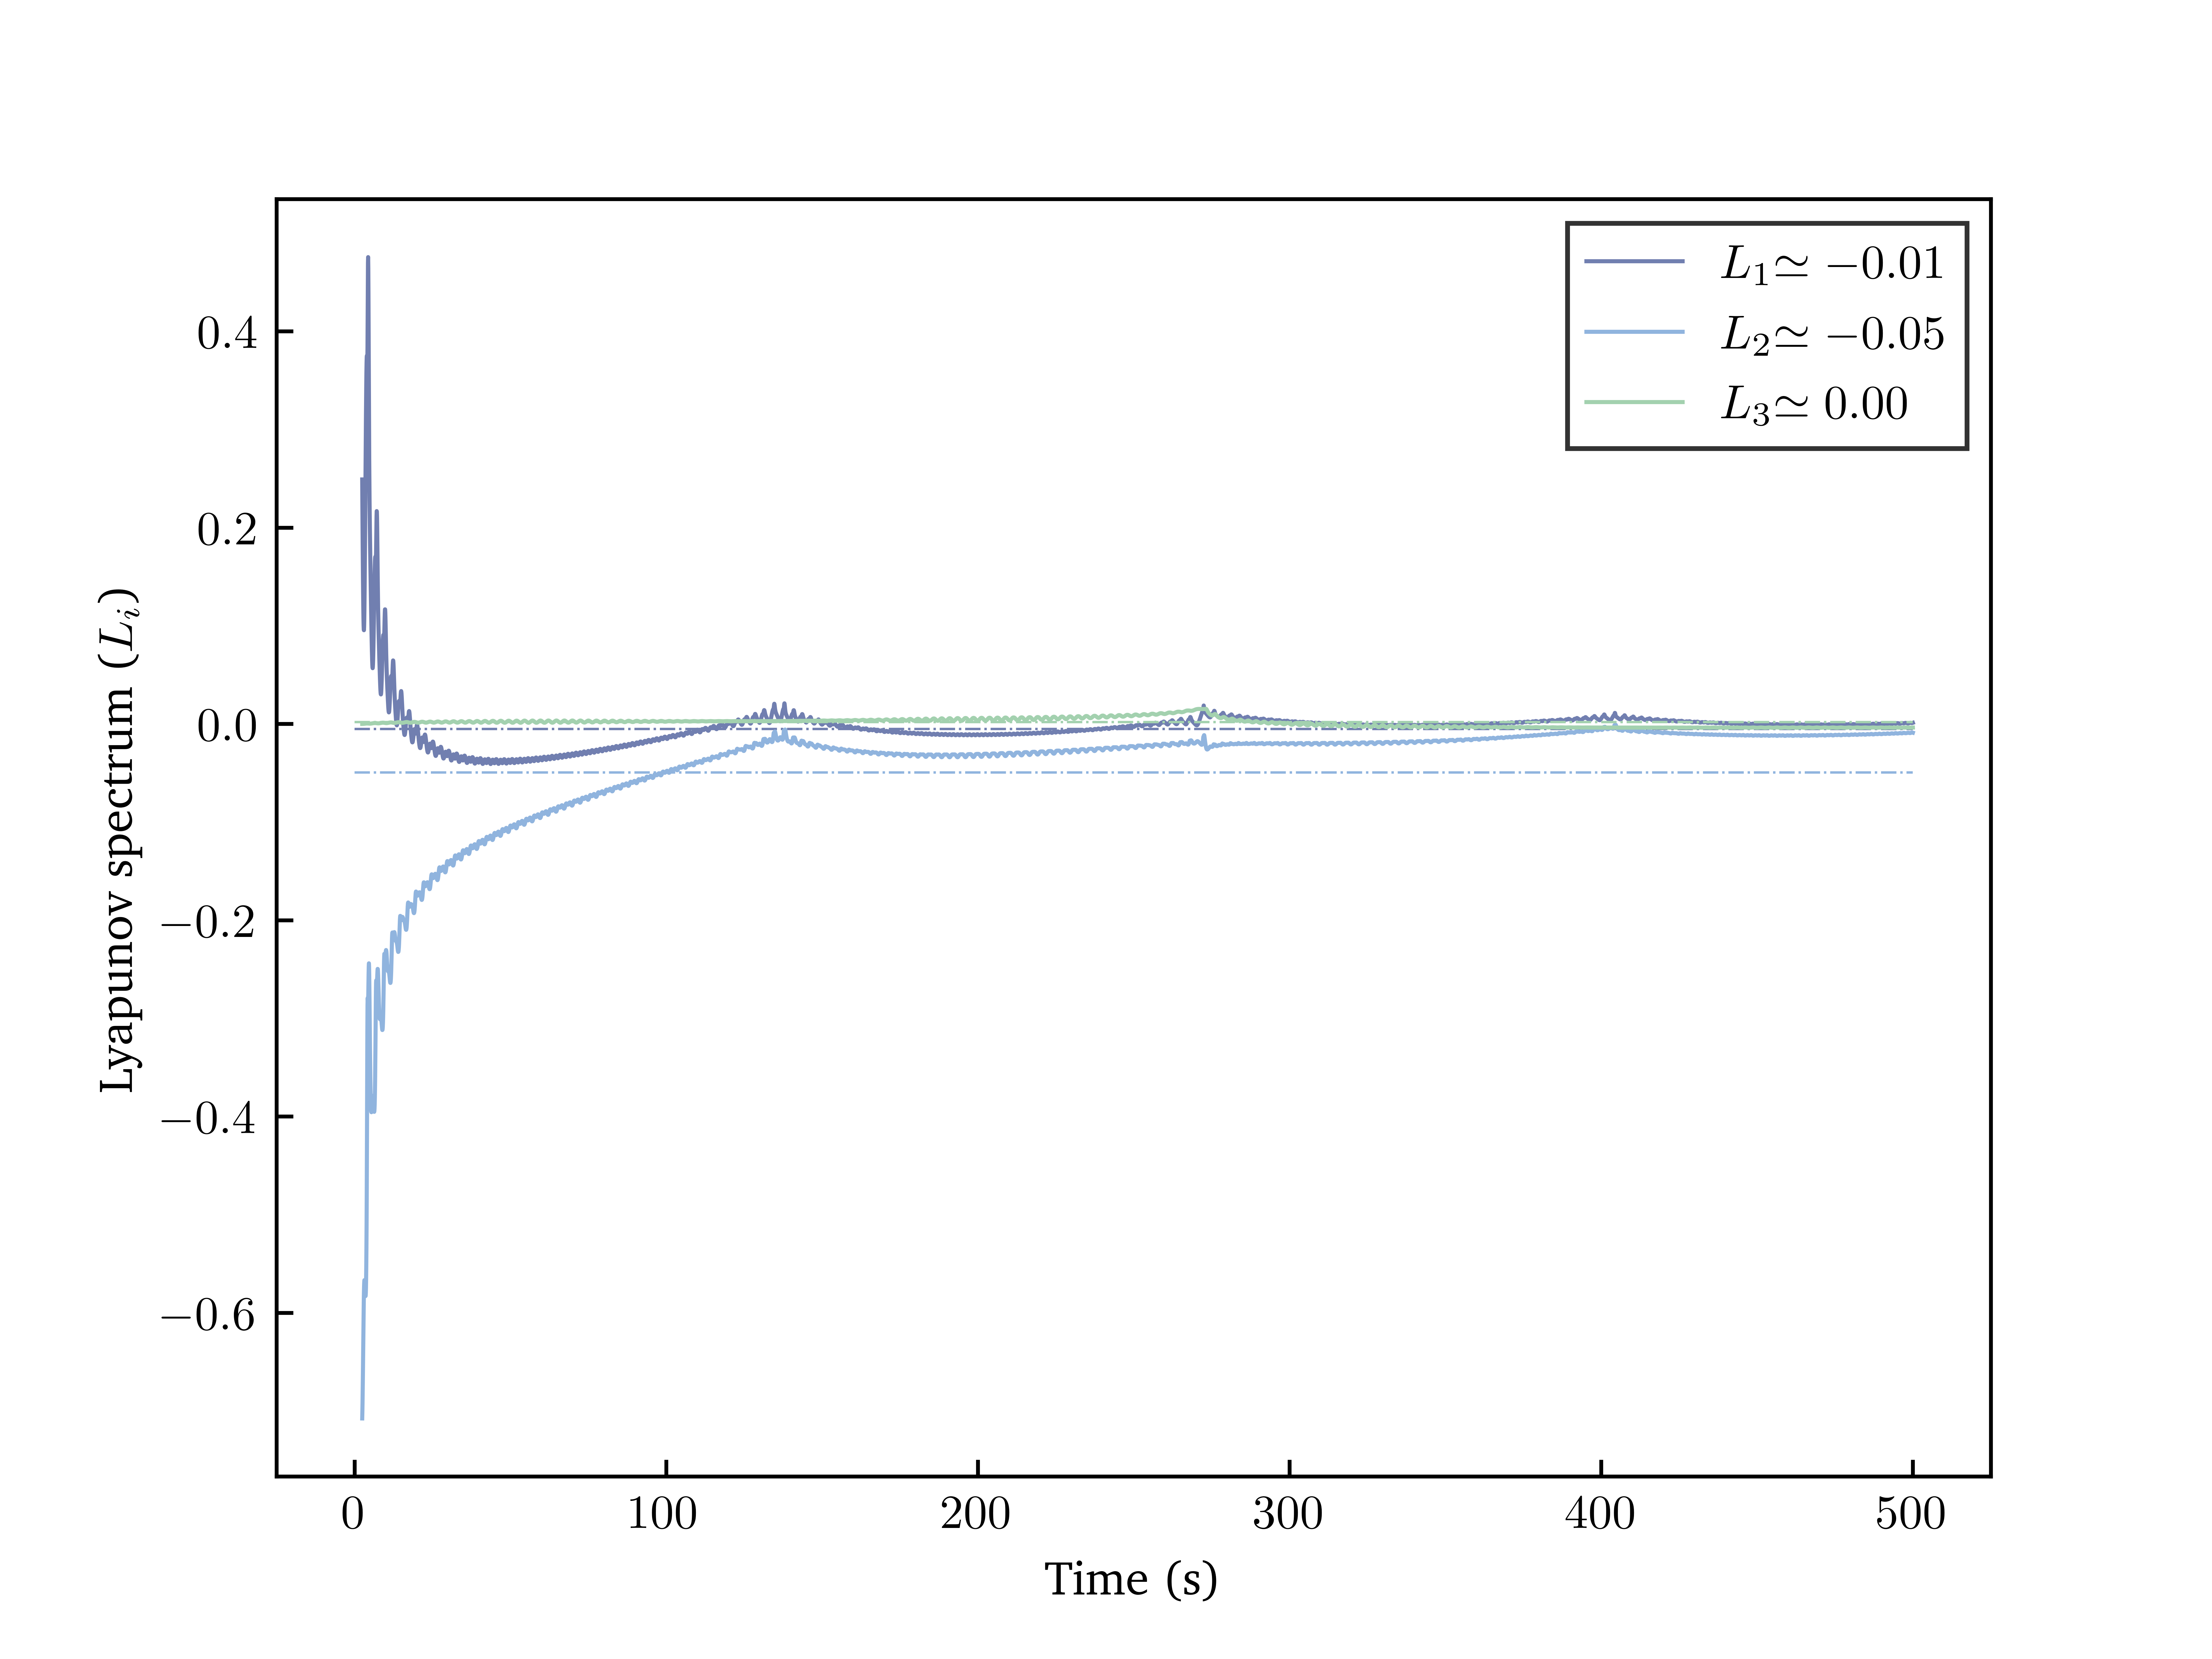
\includegraphics[scale = 0.4]{figs/lyapunovs/lyap_bouali.png}
          \subcaption{}
          \label{fig: lyap_bouali}
        \end{minipage}
        \begin{minipage}{0.49\textwidth}
          \centering
          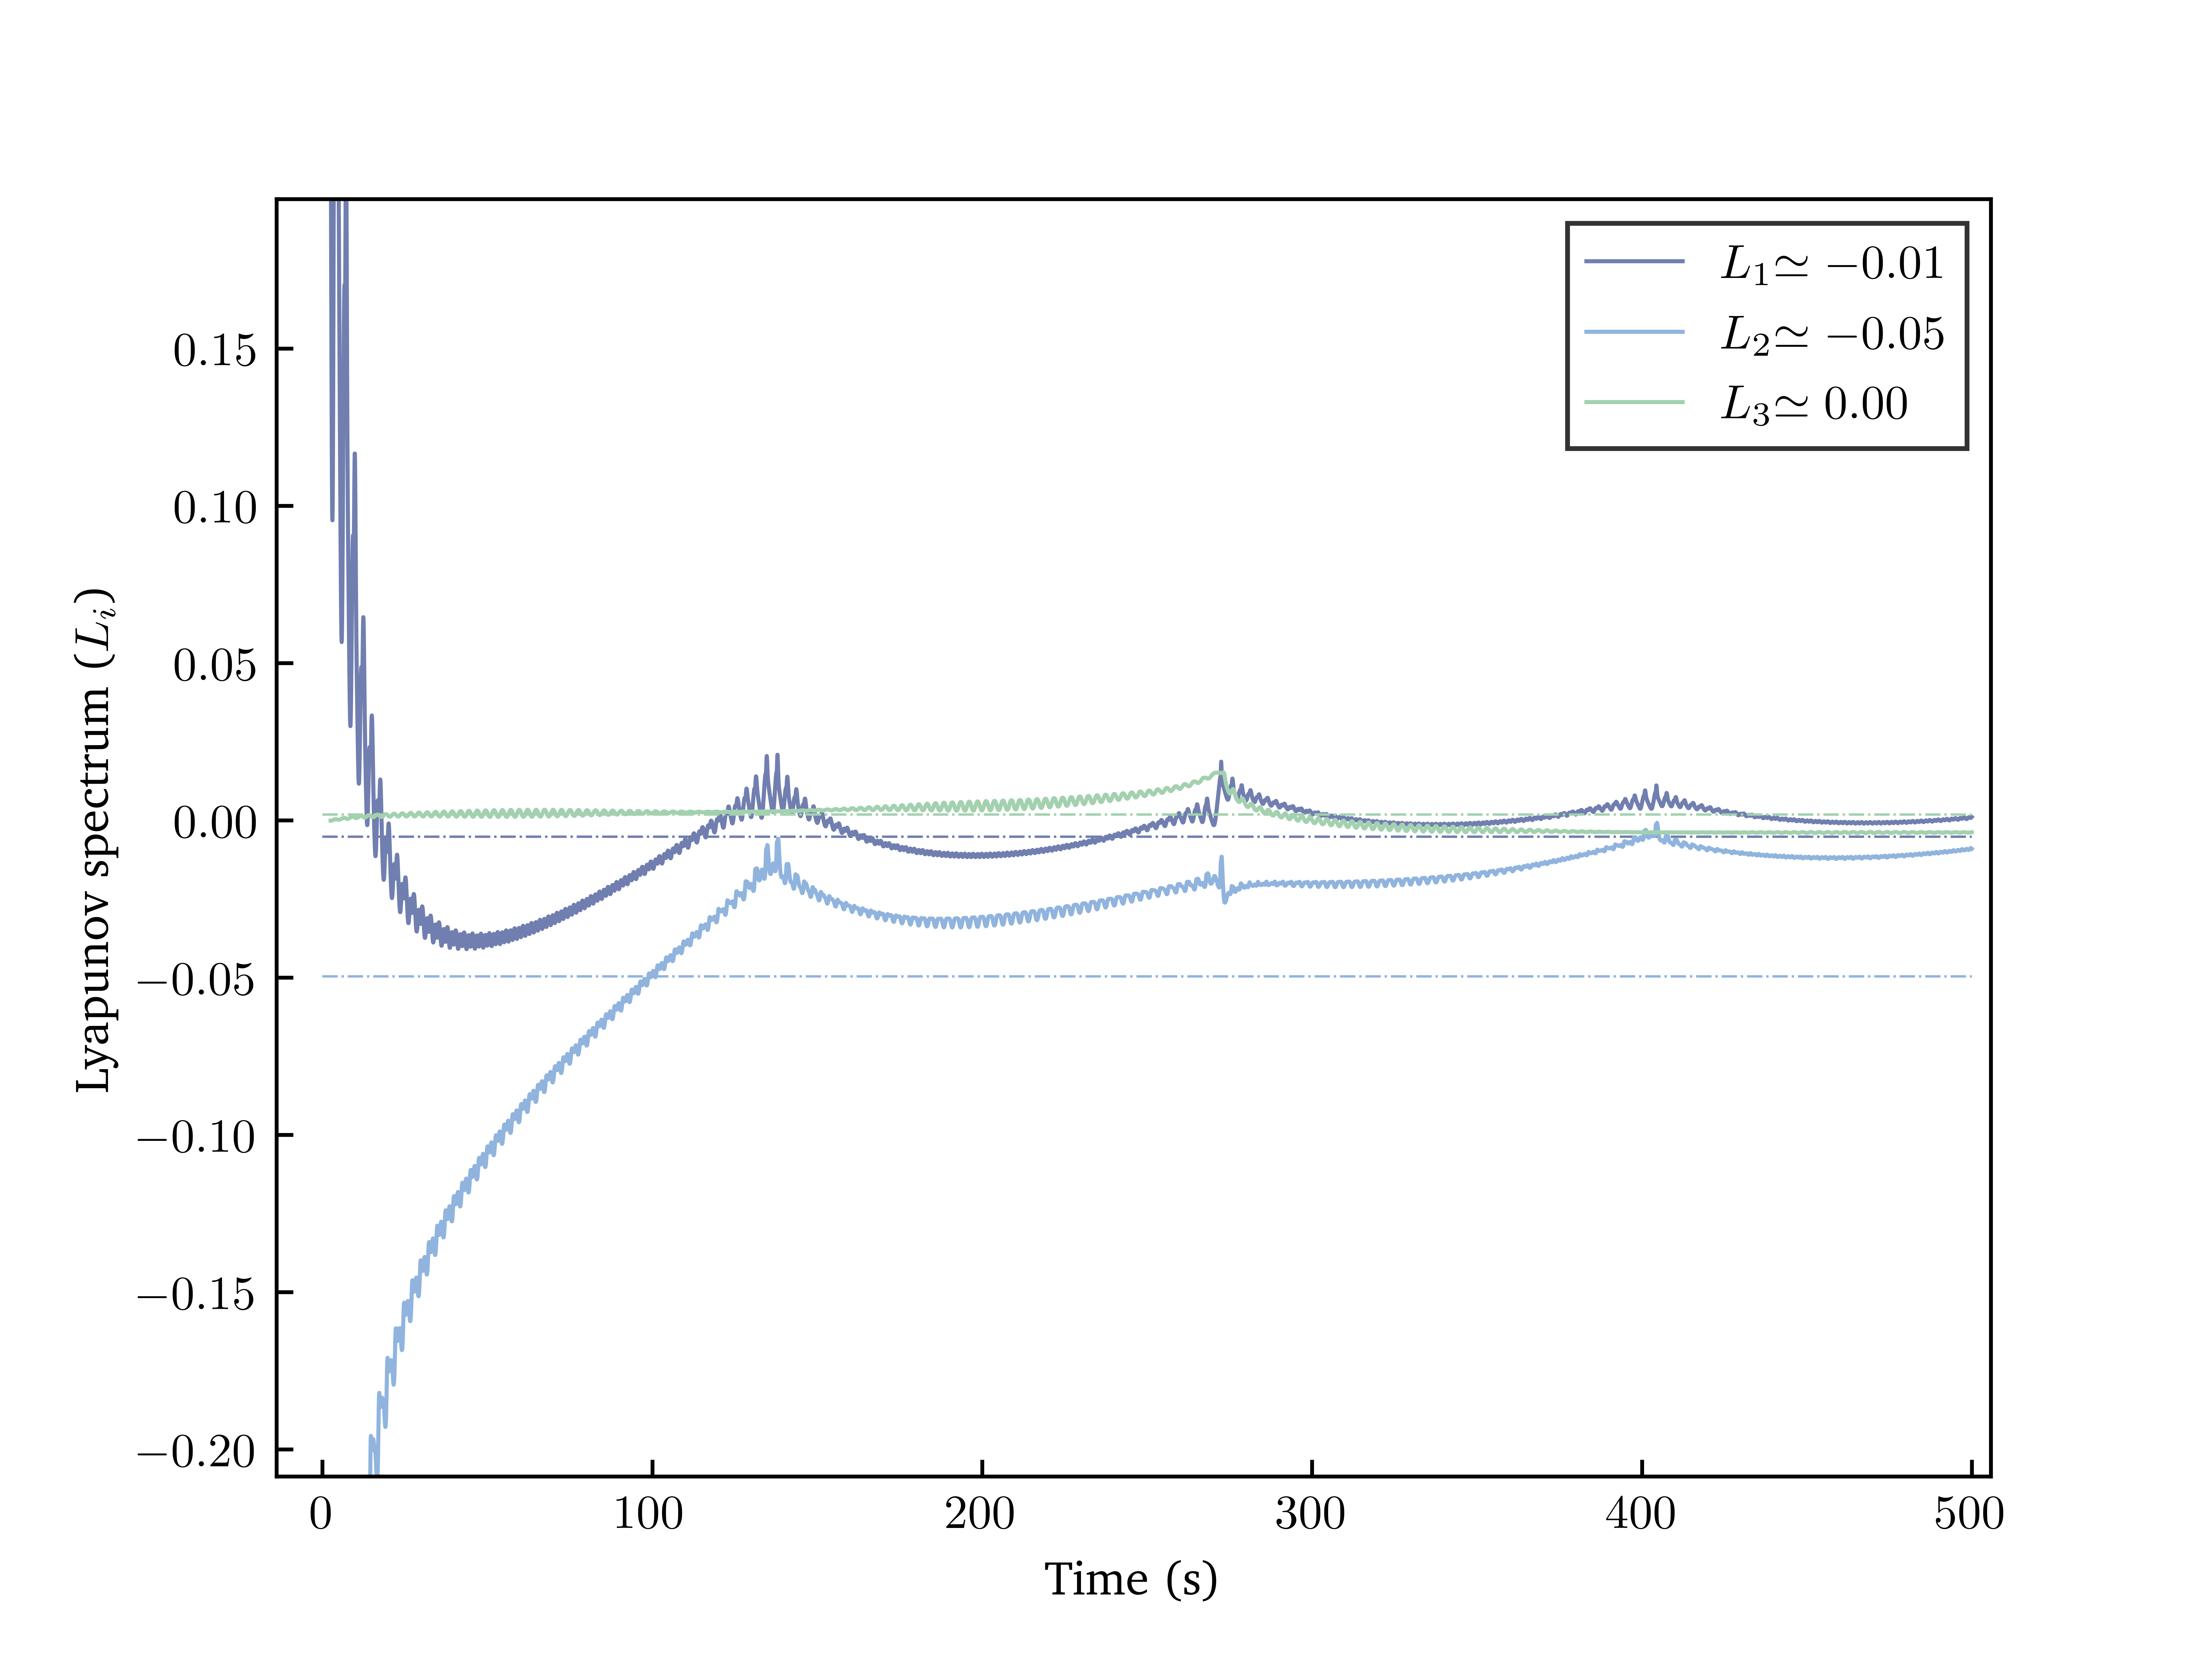
\includegraphics[scale = 0.4]{figs/lyapunovs/lyap_bouali_zoom.png}
          \subcaption{}
          \label{fig: lyap_bouali_zoom}
        \end{minipage}
        \caption{Spectre de Lyapunov ($\lambda_i\forall i\in\{1, 2, 3\}$) dans
        la simulation de l'attracteur de Bouali. (a) Spectre complet. (b) Mise
    en évidence du comportement pour les exposants $\lambda_1$, $\lambda_2$ et
$\lambda_3$ étant donnée la superposition et le bruit.}
        \label{fig : lyaps_bouali}
    \end{figure}

\twocolumngrid
